\begin{center}
    \textbf{--------- Lezione 2 - 2 ottobre 2020 ---------}
\end{center}

I sistemi operativi per dispositivi mobili condividono con i SO per i dispositivi tradizionali moltissimi aspetti concettuali.

%%%%%%%%%%%%%%%%%%%%%%%%%%% PRIMA PARTE %%%%%%%%%%%%%%%%%%%%%%%%%%%
\section{Introduzione ai SO per dispositivi mobili}
L'obiettivo dei SO per dispositivi mobili sono:
\begin{itemize}
    \item ottimizzare l'uso delle risorse
    \item semplificare l'accesso alle risorse da parte del programmatore
\end{itemize}

Una peculiarità dei SO è che le risorse sono particolarmente limitate, non solo le risorse computazionali, ma anche altre risorse come ad esempio la gestione energetica. 
Un secondo aspetto sono i vincoli real-time, ad esempio nei dispositivi mobili quando si riceve una chiamata, il SO deve far mostrare all'utente la schermata apposita. 

I SO operativi più diffusi sul mercato sono due:
\begin{itemize}
    \item iOS: SO per i dispositivi Apple. Basato su Darwin, un SO open source sul quale sono basati molti dispositivi di Apple tra cui macOS, iOS, iPadOS, watchOS, tvOS. Supporta architetture ARM ed è basato su due linguaggi: Objective C, estensione di C++ e SWIFT
    \item Android: piattaforma sviluppata da Google attraverso la Open Handset Alliance. Basato su kernel Linux, supporta architetture ARM e x86. È basato su due linguaggi: Java e Kotlin. 
    
\end{itemize}

%%%%%%%%%%%%%%%%%%%%%%%%%% SECONDA PARTE %%%%%%%%%%%%%%%%%%%%%%%%%%
\section{Gestione della memoria}
\subsection{Gestione della memoria nei dispositivi tradizionali}
Nei dispositivi tradizionali abbiamo una memoria virtuale, ogni processo sa che ha uno spazio di memoria a lui dedicato e può leggere e scrivere in quello spazio. 
Se i processi scrivessero dove vogliono, si scriverebbero uno sull'altro. 

La memoria è organizzata in pagine, in blocchi. Quando il SO si accorge che la memoria finisce, prende alcune pagine e le sposta in memoria secondaria (swap). In questo modo libera la memoria principale. Lo swap è un'operazione costosa in termini computazionali, perché il tempo di lettura/scrittura di dati da memoria secondaria è diversi ordini di grandezza maggiore rispetto a quello da memoria principale.

\subsection{Gestione della memoria nei dispositivi mobili}
Nei dispositivi mobili esiste il concetto di memoria virtuale, esiste il concetto della paginazione ma non esiste lo swapping, ovvero i dati sulla memoria principale non vengono mai spostati sulla memoria secondaria. 
\\ Quando il sistema operativo termina la memoria principale, uno o più processi vengono terminati per liberare spazio. 

Ad esempio stiamo scrivendo una mail e ci arriva una chiamata. Il SO avvia la schermata per gestire la chiamata, ma supponiamo che la memoria finisce. Il SO termina il client di posta, in questo modo però andiamo a perdere le informazioni perché una volta finita la chiamata il SO fa ripartire automaticamente il client di posta ma ciò che stavamo scrivendo è andato perso. 

La soluzione è che SO e applicazioni collaborano per nascondere all'utente la terminazione del processo. È definito un ciclo di vita dell'applicazione organizzato in eventi. Il SO richiama questi eventi e ad ogni evento l'applicazione può eseguire un codice definito dal programmatore.

\subsection{Ciclo di vita concettuale}
Per gestire questa forma di collaborazione tra SO e applicazioni, ogni SO definisce un ciclo di vita delle applicazioni che specifica quali metodi vengono richiamati, dal SO, in quali situazioni. In questo modo il programmatore può implementare i metodi che servono in una specifica applicazione. La figura mostra uno schema astratto e semplificato di un ciclo di vita di un’applicazione. Nella realtà il ciclo di vita delle applicazioni è un po’ più complicato, per permettere al programmatore di avere maggiore controllo e per evitare di svolgere operazioni non necessarie.
Nella figura i riquadri bianchi rappresentano lo stato dell'applicazione, mentre i riquadri grigi rappresentano i metodi che il SO operativo richiama quando l’applicazione cambia di stato. Gli stati sono tre: 
\begin{itemize}
    \item l’applicazione non è in esecuzione (nel senso che non esiste un processo)
    \item l’applicazione è in esecuzione ma non può essere interrotta dal SO per liberare memoria, per esempio perché sta eseguendo in foreground 
    \item l’applicazione è in esecuzione e può essere interrotta dal SO per liberare memoria (per esempio perché non è visibile e non sta eseguendo codice in background)
\end{itemize}
\begin{center}
    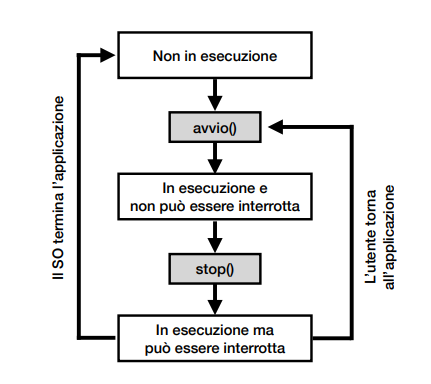
\includegraphics[width=.5\textwidth]{images/Mobile computing/2. Sistemi operativi/ciclo di vita.PNG}
\end{center}

\subsection{Ciclo di vita in Android}
Il procedimento avviene in un modo più complicato. 

Quando scriviamo un'applicazione è possibile scrivere dei metodi che gestiscano l'applicazione quando cambia di stato. In questo modo quando riceviamo una chiamata mentre stiamo scrivendo una mail, la chiamata viene messa in foreground e la mail in background. Quando l'applicazione viene messa in background viene eseguito il metodo che ha implementato il programmatore, ad esempio vengono salvati sul file il destinatario, il testo e l'oggetto della mail. Una volta terminata la chiamata, viene riaperta la mail e viene eseguito un altro metodo di cambio stato che va a leggere il file salvato in precedenza e la mail viene ripristinata.
\newpage
In Android il ciclo di vita viene associato ad un'Activity, un oggetto che rappresenta una schermata dell'applicazione.
Quando l'Activity viene avviata, vengono richiamati in ordine tre metodi: 
\begin{itemize}
    \item onCreate()
    \item onStart()
    \item onResume()
\end{itemize}
Sono questi i metodi che devono eventualmente ripristinare lo stato dell'applicazione. 
\begin{center}
    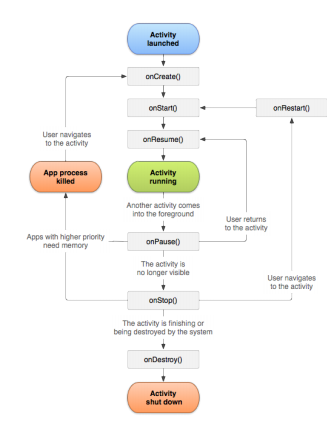
\includegraphics[width=.6\textwidth]{images/Mobile computing/2. Sistemi operativi/ciclo di vita Android.PNG}
\end{center}

\subsection{SO tradizionale}
Quando il SO necessita di memoria principale, sposta le pagine relative al processo (solo in parte o tutte) su disco. 
Queste pagine possono includere sia dati che effettivamente devono essere memorizzati (come il testo della mail), sia altri che magari non sono necessariamente da memorizzare, come ad esempio il codice dell'applicazione, le informazioni sul layout grafico (es. gli oggetti che rappresentano i pulsanti e gli altri oggetti di interfaccia), dati multimediali che non devono essere salvati perché
già disponibili su disco (es. un’immagine). 
\\ Può succedere che siano scritti su disco molti più dati di quelli che siano necessari. Questo avviene perché il SO non ha modo di sapere quali dati sia necessario salvare e quali no, in quanto questa sia un'informazione specifica alla logica dell'applicazione.

Il vantaggio  di questa soluzione è che il programmatore non si preoccupa di scrivere il codice per salvare i dati dell'applicazione. 

Nei dispositivi mobili il SO delega al programmatore l’onere di scegliere quali dati salvare e di ripristinare lo stato dell'applicazione quando questa viene fatta (ri)partire. 
\\ Abbiamo diversi svantaggi: 
\begin{itemize}
    \item il programmatore deve scrivere del codice in più per salvare e ripristinare i dati
    \item potrebbero esserci comportamenti indesiderati, come una perdita di dati, nel caso in cui il codice scritto dal programmatore contenga degli errori
    \item l'applicazione può memorizzare dati in memoria persistente anche quando non viene terminata, svolgendo così operazioni non necessarie
\end{itemize}
Tra i vantaggi invece:
\begin{itemize}
    \item l'applicazione riesce a memorizzare solo i dati strettamente necessari
    \item il SO può terminare dei processi senza dover salvare prima dei dati, perché questi sono già stati memorizzati
\end{itemize}

%%%%%%%%%%%%%%%%%%%%%%%%%%% TERZA PARTE %%%%%%%%%%%%%%%%%%%%%%%%%%%
\section{Astrazione hardware e software}
Una delle funzioni principali offerte dai SO (sia per dispositivi tradizionali che mobili) è quella di permettere al programmatore di scrivere codice che possa funzionare su dispositivi differenti. Questa funzione si chiama \textit{astrazione hardware}.
\\ Il problema dell'astrazione è più complesso rispetto ai dispositivi tradizionali ed è causato dalla frammentazione:
\begin{itemize}
    \item hardware: ci sono molti dispositivi differenti, spesso con caratteristiche molto diverse tra loro. Un utente dovrebbe verificare la disponibilità di una periferica prima di utilizzarla e prevedere un comportamento dell'app nel caso in cui non ci sia
    \item software
\end{itemize}

\subsection{Frammentazione software}
I processi interagiscono con il SO tramite chiamate dette API di SO. Queste API cambiano nel tempo quando cambia la versione del SO. Due versioni hanno alcuni metodi che possono rimanere invariati, altri che cambiano.
\\ Le API vengono introdotte al fine di: 
\begin{itemize}
    \item supportare nuove periferiche HW
    \item supportare nuovi servizi
    \item risolvere problemi delle versioni precedenti
\end{itemize}

La soluzione al problema è che il programmatore, quando sviluppa un'app, deve specificare quali versioni del SO sono supportate, indicando la più vecchia e la più recente da supportare. L'ultima versione supportata tipicamente è l'ultima rilasciata, mentre per valutare la prima dobbiamo considerare:
\begin{itemize}
    \item raggiungere il più utenti possibili
    \item maggiore è il numero di versioni che l'app deve supportare, maggiore potrebbe essere lo sforzo per realizzarla 
\end{itemize}
\begin{center}
    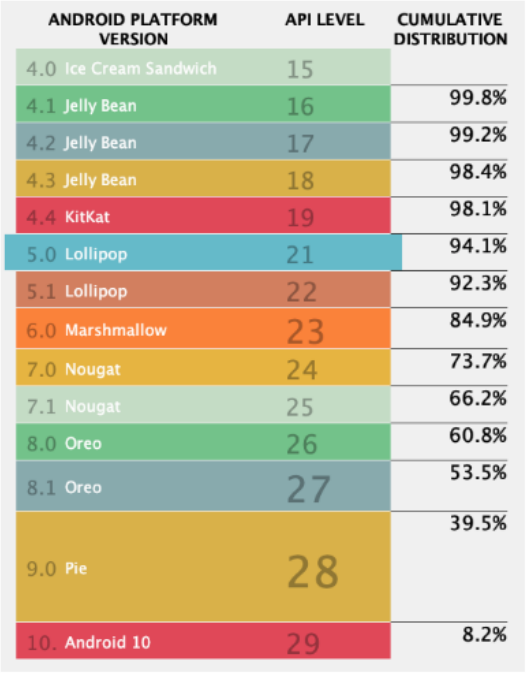
\includegraphics[width=.52\textwidth]{images/Mobile computing/2. Sistemi operativi/frammentazione sw.PNG}
\end{center}

Quando facciamo un nuovo progetto in Android, dobbiamo dire qual'è la minima versione di API che vogliamo supportare.
Se sviluppo con l'ultima versione, devo gestire solo le API 29 e so che va fatto in un'unica maniera, però vado a raggiungere l'8.2\% degli utenti.
Se scelgo la versione 4.0, diventa veramente complicato gestire il codice di tutte e quante le versioni, per questo scelgo un compromesso, come ad esempio la versione 5.0. 

Il problema è particolarmente sentito su Android perché alcuni dispositivi non permettono l'aggiornamento del SO. 

Su iOS il problema esiste ma è meno marcato. 
Ciò non vuol dire che il problema della frammentazione non ci sia. 

%%%%%%%%%%%%%%%%%%%%%%%%%%% QUARTA PARTE %%%%%%%%%%%%%%%%%%%%%%%%%%%
\section{Gestione della sincronizzazione}
I SO moderni sono multi-task, gestiscono più processi in esecuzione in contemporanea. 
Se abbiamo una CPU single core, la CPU alterna i processi facendo sembrare che i processi siano eseguiti in parallelo. Ora la maggior parte delle CPU sono multi-core ed eseguono i processi in parallelo.
L'esecuzione in parallelo non avviene solo tra singoli processi, ma all'interno del singolo processo posso avere più thread che possono essere eseguiti in parallelo. 
In questo modo abbiamo dei problemi di sincronizzazione e dobbiamo assicurare che i thread collaborino e che non rimangano in attesa di qualcosa che non succeda mai (deadlock).

Nella programmazione dei dispositivi mobili e in generale per tutti i sistemi che hanno un'interfaccia grafica, la programmazione concorrente deve essere considerata in un contesto di programmazione ad eventi.
I programmi hanno eventi che sono asincroni rispetto al codice, ad esempio il tap dell'utente sullo schermo.
Non sappiamo quando accadrà l'evento, ma quando accade verrà eseguito un metodo. 

Nei dispositivi mobili in ogni processo esiste un solo thread, \textit{main thread}, che può modificare l'interfaccia grafica e gestire gli eventi generati dall'interfaccia utente. 
Gli altri thread secondari sono chiamati \textit{background thread} e non possono modificare l’interfaccia utente altrimenti il sistema genera un’eccezione a runtime.
Il main thread non deve rimanere bloccato, altrimenti non riuscirebbe a gestire l'interfaccia grafica. 

Abbiamo ad esempio un'app che, al tocco su un pulsante, fa una comunicazione di rete. 
L'utente tocca il pulsante, il SO genera un evento che viene gestito dal thread principale e l'app effettua una comunicazione di rete. La chiamata è bloccante perché il thread rimane in attesa della risposta. Nessun altro thread può modificare la GUI perché il thread è in attesa.

Dobbiamo far si che il main thread vada a generare un altro thread (thread secondario) che gestisca le operazioni che richiedono I/O e la computazione CPU bound. 
Quando il thread secondario termina non può aggiornare l'interfaccia grafica e deve far intervenire il main thread in quanto solo lui possa aggiornare. 
In questo caso abbiamo un problema di sincronizzazione. 
Questo può avvenire in vari modi:
\begin{itemize}
    \item costrutti di sincronizzazione di basso livello: come wait, notify o i semafori. Sono complessi da utilizzare, soggetti ad errore e difficili da testare.
    \item costrutti di sincronizzazione di alto livello: introdotti per semplificare la gestione del codice nei casi tipici della gestione degli eventi, come ad esempio un thread secondario che può richiedere al thread principale di eseguire del codice.

    \item chiamate asincrone: in alcuni casi si scrivono metodi non bloccanti che al loro interno eseguono il codice bloccante. 
    
\end{itemize}

\subsection{Errori e soluzioni}
\subsubsection{Errori}
\textbf{Algoritmo 1. }Esempio di errore: il main thread fa una chiamata bloccante
\begin{Java}
    //Codice eseguito quando l'utente preme sul pulsante
    result = sendRequest("myServer.com");
    myTextField.setText(result);
\end{Java}
\textbf{Algoritmo 2. }Esempio di errore: un thread secondario prova a modificare l’interfaccia grafica
\begin{Java}
    //Codice eseguito quando l'utente preme sul pulsante
    Crea un thread secondario che faccia questo {
        result = sendRequest("myServer.com");
        myTextField.setText(result);
    }
\end{Java}

\textbf{Algoritmo 3. }Esempio di errore: il main thread prova ad utilizzare il risultato della chiamata di rete prima che questo sia disponibile
\begin{Java}
    //Codice eseguito quando l'utente preme sul pulsante
    Crea un thread secondario che faccia questo {
        result = sendRequest("myServer.com");
    }
    myTextField.setText(result);
\end{Java}
\subsubsection{Soluzioni}
\textbf{Algoritmo 4. }Soluzione: uso di costrutti di sincronizzazione di alto livello
\begin{Java}
    //Codice eseguito quando l'utente preme sul pulsante
    Crea un thread secondario che faccia questo {
        result = sendRequest("myServer.com");
        esegui questo codice nel thread principale {
            myTextField.setText(result);
        }
    }
\end{Java}
\textbf{Algoritmo 5. }Soluzione: uso delle chiamate asincrone
\begin{Java}
    //Definiamo prima questa chiamata
    func manageResult(result) {
        myTextField.setText(result);
    }
\end{Java}
\begin{Java}
    //Codice eseguito quando l'utente preme sul pulsante
    sendRequestAsync("myServer.com", manageResult);
\end{Java}

\section{Gestione del background}
Nei dispositivi tradizionali, quando scriviamo app non ci poniamo il problema se il codice viene eseguito in foreground o in background.
Il programmatore non deve fare nulla per fare funzionare il codice in background e non c'è differenza tra codice che viene eseguito in background e in foreground.

Nei dispositivi mobili c'è una differenza. Anche i dispositivi mobili permettono il multitasking, oltre al processo in foreground possono essere in esecuzione anche processi in background. 
\\ I processi in background hanno un forte impatto sulle performance delle app in foreground e sulla durata della batteria. Per questo i SO per dispositivi mobili pongono delle limitazioni all'esecuzione in background. 
L'ideale sarebbe non fare eseguire del codice in background ma questo non è possibile perché ci sono sistemi di messaggistica che devono poter ricevere messaggi anche quando l'app non è in foreground.
Un altro esempio ne è un sistema che deve riprodurre musica anche in background. 

In tutti i casi in cui un’applicazione necessita di ricevere dati in modo asincrono via rete (es: sistema di messaggistica), viene adottato un protocollo di comunicazione chiamato \textit{push notification}, che permette all'applicazione di non dover eseguire codice in background.

In altri casi come l'app di musica, non è possibile evitare di eseguire il codice in background. 

\subsection{Background in iOS}
Apple ha da sempre avuto un approccio molto restrittivo rispetto al background, le applicazioni non possono eseguire codice arbitrario in background se non in risposta ad alcuni specifici eventi. 
\\ Ad esempio abbiamo un'applicazione che ha bisogno di conoscere la posizione dell'utente anche in background, può registrarsi per essere notificata dal SO quando la posizione cambia. 
Il SO ogni volta che osserva un cambio di posizione, notifica l'app che ha poi un tempo ridotto per gestire l'evento e se non lo gestisce entro questo tempo, il SO termina il processo. 

\subsection{Background in Android}
Ci sono due categorie di processi in background: 
\begin{itemize}
    \item quelli che hanno effetti immediati sull'utente (es: la musica, app che mostrano informazioni saltuariamente all'utente, come le app di navigazione) possono eseguire codice arbitrario anche in background 
    \item quelli che non hanno effetti immediati (es: compatimento di un database) possono eseguire codice solo attraverso uno strumento (SW) di pianificazione delle attività: il SO eseguirà quelle attività quando possibile (es: quando disponibile una connessione WiFi, quando la batteria è carica, ecc.)
\end{itemize}

